\section{Implementación y evaluación de las técnicas}

% (Aquí no te pongo límite de páginas. Explícalo como quieras ya que es la parte en la que tienes que explicar el trabajo técnico que has realizado.)

\subsection{Detalles de la implementación de las técnicas de DL aplicadas}

% (Esto sería parte práctica)
% una especie de bitácora sin hablar en primera persona

{\color{red} \textbf{!!! TODO}}

\subsection{Evaluación de las técnicas}

Se han entrenado dos versiones de YOLO: la versión 3 y la versión 3 tiny. Inicialmente se entrenó únicamente la versión 3, pero al ejecutarla en un dispositivo móvil se observó que el rendimiento lo hacía inutilizable, es este el motivo por el cual que se ha entrenado la versión tiny.

Para cada una de estas versiones se han entrenado varios modelos con distintos tamaños de red, por dos motivos principalmente: por una cuestión de rendimiento a la hora de ejecutar el modelo en un dispositivo móvil y por analizar cómo varía la precisión del modelo cambiando el tamaño de la red.

Además se han utilizado distintos conjuntos de entrenamiento para entrenar todas las variantes del modelo. El primero de los conjuntos de entrenamiento se corresponde con el conjunto íntegro original (denominado \textit{completo}). Los resultados obtenidos con este conjunto de entrenamiento obtuvieron unos valores bajos para la métrica \textit{AP}, y tras analizar los motivos, se observó que había una gran cantidad de socavones demasiado pequeños que podían ser los causantes malos resultados. Por este motivo, se han utilizado dos conjuntos de entrenamiento adicionales aplicando filtros sobre los socavones. En el primero de estos conjuntos de entrenamiento adicionales se han filtrado los socavones con tamaño superior a 75x30 píxeles (denominado \textit{filtro 75x30}) y en el segundo se han filtrado los socavones con tamaño superior a 100x40 píxeles (denominado \textit{filtro 100x40}). Para cada uno de estos conjuntos de entrenamiento adicionales se ha creado también su correspondiente conjunto de evaluación aplicando el mismo filtro.

Con todos los modelo resultantes obtenidos se ha realizado una doble evaluación. Por un lado se han evaluado con los conjuntos de test correspondientes para cada uno de los conjuntos de entrenamiento (resultados en la figura \ref{fig:evaluationoriginal}). Y por otro lado se han evaluado con un conjunto de imágenes generado para este proyecto (resultados en la figura \ref{fig:evaluationcustom}). Este conjunto de evaluación (denominado \textit{propio}) se compone de unas 30 imágenes de 4032x3024 píxeles, con unos 60 socavones en total, obtenido desde la acera (a diferencia del original que fue obtenido desde el coche) y compuesto por fotos realizadas en España (a diferencia del original que fueron realizadas en Sudáfrica).

\begin{figure}[H]
	\centering
	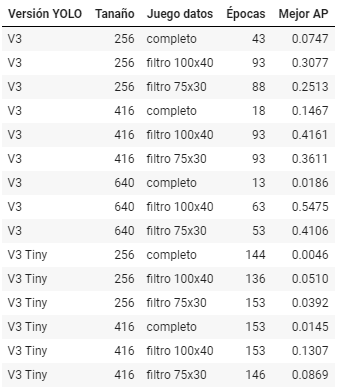
\includegraphics[width=0.6\linewidth]{images/evaluation_original.png}
	\caption{Resultados obtenidos con los conjuntos de evaluación originales}
	\label{fig:evaluationoriginal}
\end{figure}

\begin{figure}[H]
	\centering
	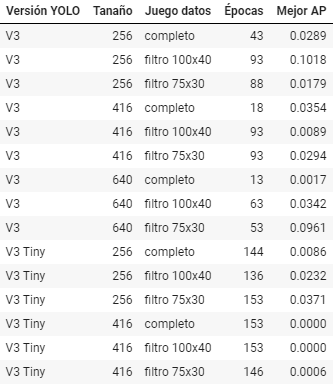
\includegraphics[width=0.6\linewidth]{images/evaluation_custom.png}
	\caption{Resultados obtenidos con el conjunto de evaluación propio}
	\label{fig:evaluationcustom}
\end{figure}